% !TeX program = xelatex
% !TeX program = xelatex

\documentclass[12pt]{article}

\usepackage{lineno,changepage,lipsum}
\usepackage[colorlinks=true,urlcolor=blue]{hyperref}
\usepackage{fontspec}
\usepackage{xeCJK}
\usepackage{tabularx}
\setCJKfamilyfont{chanto}{AozoraMinchoRegular.ttf}
\setCJKfamilyfont{tegaki}{Mushin.otf}
\usepackage[CJK,overlap]{ruby}
\usepackage{hhline}
\usepackage{multirow,array,amssymb}
\usepackage[croatian]{babel}
\usepackage{soul}
\usepackage[usenames, dvipsnames]{color}
\usepackage{wrapfig,booktabs}
\renewcommand{\rubysep}{0.1ex}
\renewcommand{\rubysize}{0.75}
\usepackage[margin=50pt]{geometry}
\modulolinenumbers[2]

\usepackage{pifont}
\newcommand{\cmark}{\ding{51}}%
\newcommand{\xmark}{\ding{55}}%

\definecolor{faded}{RGB}{100, 100, 100}

\renewcommand{\arraystretch}{1.2}

%\ruby{}{}
%$($\href{URL}{text}$)$

\newcommand{\furigana}[2]{\ruby{#1}{#2}}
\newcommand{\tegaki}[1]{
	\CJKfamily{tegaki}\CJKnospace
	#1
	\CJKfamily{chanto}\CJKnospace
}

\newcommand{\dai}[1]{
	\vspace{20pt}
	\large
	\noindent\textbf{#1}
	\normalsize
	\vspace{20pt}
}

\newcommand{\fukudai}[1]{
	\vspace{10pt}
	\noindent\textbf{#1}
	\vspace{10pt}
}

\newenvironment{bunshou}{
	\vspace{10pt}
	\begin{adjustwidth}{1cm}{3cm}
	\begin{linenumbers}
}{
	\end{linenumbers}
	\end{adjustwidth}
}

\newenvironment{reibun}{
	\vspace{10pt}
	\begin{tabular}{l l}
}{
	\end{tabular}
	\vspace{10pt}
}
\newcommand{\rei}[2]{
	#1&\textit{#2}\\
}
\newcommand{\reinagai}[2]{
	\multicolumn{2}{l}{#1}\\
	\multicolumn{2}{l}{\hspace{10pt}\textit{#2}}\\
}

\newenvironment{mondai}[1]{
	\vspace{10pt}
	#1
	
	\begin{enumerate}
		\itemsep-5pt
	}{
	\end{enumerate}
	\vspace{10pt}
}

\newenvironment{hyou}{
	\begin{itemize}
		\itemsep-5pt
	}{
	\end{itemize}
	\vspace{10pt}
}

\date{\today}

\CJKfamily{chanto}\CJKnospace
\author{Tomislav Mamić}

\begin{document}
	\dai{\furigana{原稿用紙}{げんこうようし}の使い方}
	
	\fukudai{Izgled papira}
		
	\begin{wrapfigure}[11]{r}{.25\textwidth}
		\centering
		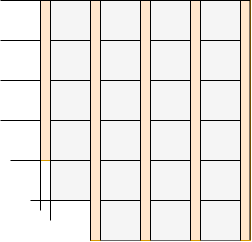
\includegraphics[width=.25\textwidth]{017_pisanje_res/a1.png}
		\caption{izgled papira}
	\end{wrapfigure}

	Na desnoj strani prikazana je rešetka 原稿用紙 papira, preciznije gornji desni kut. Kvadratna polja u koja se upisuju znakovi (マス) složena su u stupce odvojene uskim okomitim prostorom koji služi za upisivanje čitanja težih znakova (ふりがな).
	
	Papir je položen vodoravno, a tekst se piše okomito prema dolje, s desne strane prema lijevoj. Osim u jednoj iznimnoj situaciji, svaki je znak, uključujući i interpunkciju, smješten u svoje polje.
	
	\begin{wrapfigure}[11]{r}{.25\textwidth}
		\centering
		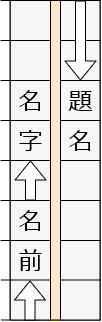
\includegraphics[width=.1\textwidth]{017_pisanje_res/a2.png}
		\caption{naslov i ime}
	\end{wrapfigure}
	
	\fukudai{\furigana{題名}{だいめい}・名前\ - naslov i ime}

	Naslov teksta piše se u prvi stupac, tako da se preskoče prva dva ili tri polja. Ako naslov ne stane u prvi stupac, onda je to loš naslov. Ime se piše u sljedeći stupac, tako da se piše prvo (iznad) prezime (名字), a ispod ime (名前). Između imena i prezimena ostavlja se jedno prazno polje, a ime završava jedno polje prije kraja stupca.
		
	\fukudai{\furigana{段落}{だんらく}\ - odlomci}
		
	Odlomke obavezno započinjemo prelaskom u novi red, tako da preskočimo prvo polje (Slika 3). Ako pišemo vodoravno, logika je identična onoj u hrvatskom jeziku.

	\fukudai{Mali znakovi}
	
	Pišu se u desnu stranu polja, s tim da je okomito poravnanje na sredini (Slika 4). Možda se čini kao traćenje prostora, ali odnos veličine znaka i polja čini raspoznavanje malih i velikih znakova vrlo laganim.
	
	\fukudai{\furigana{句読点}{くとうてん}\ - točka i zarez\footnotemark[1]}
	
	\footnotetext[1]{U formalnom pisanju upitnike, uskličnike i ostale zapadne prljavštine treba izbjegavati.}
	
	Točku i zarez pišemo u gornji desni kut polja osim kad riječ prije završava točno na kraju reda (Slika 4). Kako ne bismo pisali samo točku ili zarez u novi red, dopušteno ih je napisati u donji desni kut zadnjeg polja, ili desno odmah ispod linije. I jedan i drugi način pisanja su dopušteni i točni.
	
	\newpage
	
	\fukudai{\furigana{会話文}{かいわぶん}\ - monolog i dijalog}
	
	\begin{wrapfigure}{r}{.3\textwidth}
		\centering
		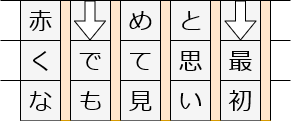
\includegraphics[width=.3\textwidth]{017_pisanje_res/a3.png}
		\caption{odlomci}
	\end{wrapfigure}

	Kao što smo dosad već sigurno primijetili, u japanskom su tekstu citati obuhvaćeni ćoškastim "zagradama" (「」). Iako su po izvornom imenu dosl. \textit{ključaste zagrade}\ (かぎかっこ), zapravo upotrebom odgovaraju hrvatskim navodnicima.
	
	Kad se pišu okomito, otvoreni navodnik ima ćošak gore desno, a zatvoreni dolje lijevo - rotiraju zajedno s papirom. S papirom rotiraju i sve "prave" zagrade, kao i oznaka dugog samoglasnika iz katakane (ー), ali \textbf{ne} broj 1 (一). Ovo je zamka.
	
	Kad pišemo linije monologa ili dijaloga likova, pišemo ih u ovim navodnicima. Obavezan je prelazak u novi stupac, nakon čega je prvi znak u sljedećem stupcu otvoreni navodnik. Ako se citat proteže kroz više stupaca, u svakom sljedećem stupcu preskačemo prvo polje (Slika 5).
	
	\begin{wrapfigure}{r}{.25\textwidth}
		\centering
		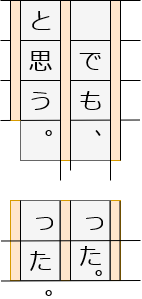
\includegraphics[width=.15\textwidth]{017_pisanje_res/a5.png}
		\caption{interpunkcija}
	\end{wrapfigure}

	Kad završavamo govor likova, gotovo se uvijek na kraju nalaze i točka i zatvoreni navodnik. U tom ih je slučaju u redu pisati zajedno, tako da je točka gore desno, a ćošak navodnika dolje lijevo. U (veoma nesretnom) slučaju kada citat završava na kraju stupca, točku i zatvoreni navodnik pišemo zajedno ispod stupca (Slika 6).
	
	Ponekad likovi u govoru navode ime ili naglašavaju neku riječ koja bi inače bila u navodnicima. U tom se slučaju koriste dvostruki navodnici\\ (『』・二重かっこ). Osim što su nevjerojatna gnjavaža za pisanje rukom, koriste se na isti način kao jednostruki.
	
	Za one kojima dvije razine gniježđenja nisu dovoljne, preporučio bih neki programski jezik s jedva čitljivom sintaksom, recimo C.
	
	\begin{wrapfigure}{l}{.25\textwidth}
		\centering
		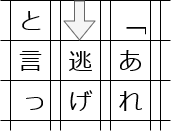
\includegraphics[width=.2\textwidth]{017_pisanje_res/b1.png}
		\caption{početak citata}
	\end{wrapfigure}
	\begin{wrapfigure}{l}{.25\textwidth}
		\centering
		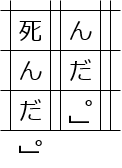
\includegraphics[width=.16\textwidth]{017_pisanje_res/b2.png}
		\caption{kraj citata}
	\end{wrapfigure}

\end{document}